\section{Approach}
\label{sec:approach}

\emph{Here, you will establish a hypothesis and explain how you seek to apply your knowledge to validate or refute the hypothesis.  Propose an experiment.  Describe it in enough detail that a classmate could replicate what you did simply by reading this report. Write out your approach as a set of numbered steps. A well-labeled schematic drawing is required in addition to your text. Include relevant photos of your setup. Photos are not a substitute for a schematic! What do you expect to see when you take data?  What trends do you expect? State your assumptions clearly.}

In order to determine the relationship between air speed and weight, we set up an experiment in which we repeatedly fly the same bird on the same flight path with varying weights. In short, the independent variable here is the weight carried by the bird, and the dependent (measured) variable is the flight time from the starting point to the end. The steps we took during the experiment are as follows.

\begin{enumerate}
\item Flash the flightpath.brd onto the AtSwallow
\item Place a 30g worm 100 feet away. The worm should be in direct line-of-sight of the bird. This will entice the bird to travel in this direction.
\item Load a standard packet with a set amount of data.
\item Attach packed to bird.
\item Hold the bird such that it faces directly opposite of the intended flightpath.
\item Release the bird.
\item Using a stopwatch, measure the time from release to the bird getting the worm.
\item Repeat steps 4 and 5 ten times for each weight.
\end{enumerate}

Figure~\ref{fig:schematic} shows a schematic diagram of the experimental setup. Note that it is important that the environment is controlled between experiments; all experiments were done in similar weather conditions, on the same day, within an hour of each other. Worm size was kept constant(within 10 milligrams of target mass), as smaller worms are less attractive to the birds.  Our initial plan was to conduct double-blind trials.  This turned out to be a mistake.  Blindfolding the sparrows was difficult and negatively impacted their flying patterns.  And blindfolding the minions conducting the experiment resulted in all matter of confusion.  We thus abandoned our initial approach and proceeded blindfold-less.

\begin{figure}[h]
\centering
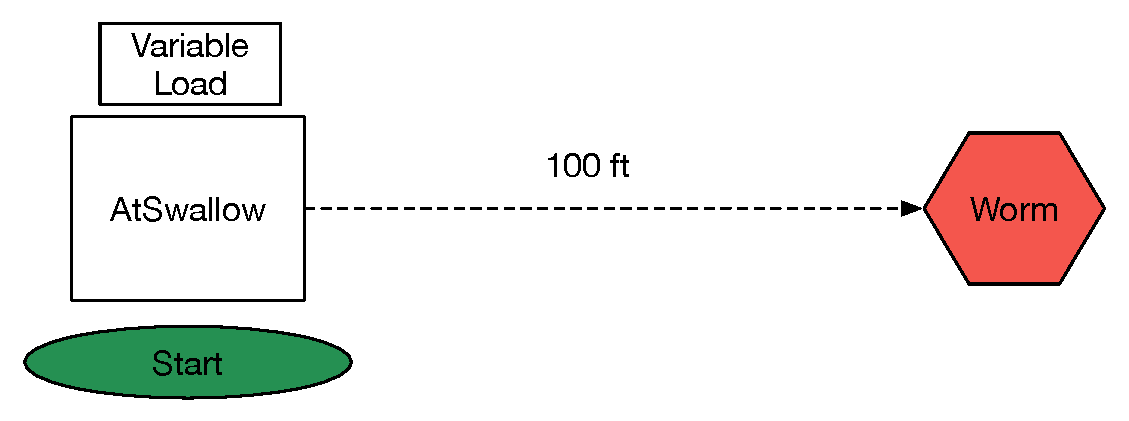
\includegraphics[width=0.4\textwidth]{Schematic}
\caption{The experiment. Not drawn to scale.}
\label{fig:schematic}
\end{figure}


\begin{figure}[h]
\centering
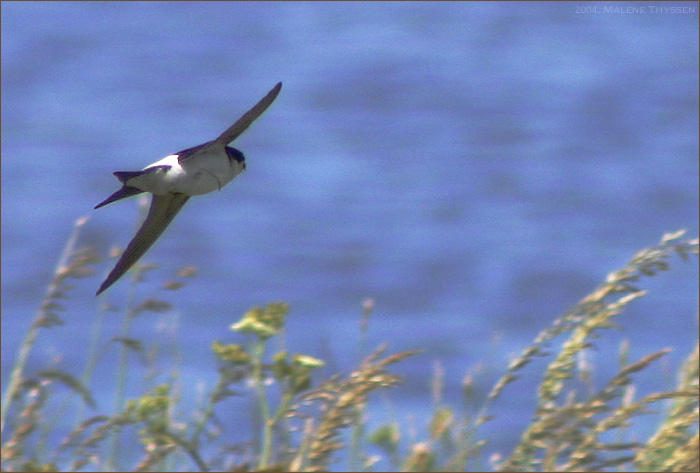
\includegraphics[width=0.3\textwidth]{experiment}
\caption{Swallow in the middle of an experiment}
\label{fig:experiment}
\end{figure}

\subsection{Assumptions}

\begin{tightitem}
\item We assume the SI system of units for all of our measurements and analysis.

\item We assume that the gravitational effects on the swallow are constant.  The governing equation, of course, is

\begin{equation}
\label{eqn:weight}
F_{gravity} = \frac{g m_{1} m_{2}}{r^2}
\end{equation}

where $F_{gravity}$ is the gravitational force [newtons] acting upon the swallow, $g$ again is the gravitational constant, $m_{1}$ is the mass of the earth [kg], $m_{2}$ is the mass of the swallow, and $r$ is the distance [m] between the centers-of-mass of the swallow and the earth.

\item We assume that the swallow will fly trajectories such that $r$'s variation would result in an insignificant variation of $F_{gravity}$.

\item We know that air-speed and velocity are different concepts (air-speed is a scalar quantity while velocity is a vector quantity).  And what we \emph{mean} is that the creature's air-speed is the magnitude of the velocity vector.  But I'm the king and I make the rules.  So I will continue to say air-speed velocity, and I expect you good subjects to smile and nod. OK?

\item We ignore relativistic effects as we are studying a sub-sonic species.  As Einstein showed, the laden-ness (mass) of our subject swallows would increase without bound as the creatures approach the speed of light.  But if we could get our swallows to move that fast, our latency and bandwidth problems would be over.  So let's be realistic.

\item We do not seek to account for the so-called \emph{birdie-birdie-in-the-sky} mass-flow phenomenon.
\end{tightitem}
